\documentclass[spanish,a4paper,11pt,twoside]{report}

%%%%%%%%%%%%%%%%%%%%%%%%%%%%%%%%%%%%%%%%%%%%%%%%%%%%%%%%%%%%%%%%%%%%%%%%%%%%%%%
\usepackage[dvips]{graphicx}
\usepackage[dvips]{epsfig}
%\usepackage[latin1]{inputenc}
\usepackage[utf8]{inputenc}
\usepackage[spanish]{babel}
\usepackage{alltt}
\usepackage{algorithm}
\usepackage{algorithmic}
\usepackage{multirow}

%
\usepackage{listings}
\usepackage{color}

\lstloadlanguages{Python,C,HTML}
\lstset{
  language=Python,                      % C,Fortran,XML
  basicstyle=\small,             % Listados en small
  keywordstyle=\color{red},             % Palabras clave en rojo
  identifierstyle=\ttfamily,
  escapeinside={(*@}{@*)},
  commentstyle=\color{blue},            % comentarios en azul
  stringstyle=\color{green},            % cadenas en verde
  showstringspaces=false,
  frame=tb,
  captionpos=b,
  framextopmargin=2pt,
  framexbottommargin=2pt,
  framesep=0pt,
  belowskip=0pt,
  aboveskip=0pt,
  belowcaptionskip=0pt,
  abovecaptionskip=0pt,
  stepnumber=2,                                         % Opciones de lineas y etiquetas
  numberstyle=\small,
  numbersep=5pt,
  tabsize=1
}


%%%%%%%%%%%%%%%%%%%%%%%%%%%%%%%%%%%%%%%%%%%%%%%%%%%%%%%%%%%%%%%%%%%%%%%%%%%%%%%

\newcommand{\SONY}{{\sc Sony}}
\newcommand{\MICROSOFT}{{\sc Microsoft}}
\newcommand{\GCC}{\textsf{\textsc{G}CC}}
\newcommand{\INTEL}{\textsf{\textsc{I}ntel}}

%%% Traducimos el pseudocodigo
\renewcommand{\algorithmicwhile}{\textbf{mientras}}
\renewcommand{\algorithmicend}{\textbf{fin}}
\renewcommand{\algorithmicdo}{\textbf{hacer}}
\renewcommand{\algorithmicif}{\textbf{si}}
\renewcommand{\algorithmicthen}{\textbf{entonces}}
\renewcommand{\algorithmicrepeat}{\textbf{repetir}}
\renewcommand{\algorithmicuntil}{\textbf{hasta que}}
\renewcommand{\algorithmicelse}{\textbf{en otro caso}}
\renewcommand{\algorithmicfor}{\textbf{para}}

%\newcommand{\RETURN}{\textbf{retornar} }
\newcommand{\RET}{\STATE \textbf{retornar} }
\newcommand{\TO}{\textbf{hasta} }
\newcommand{\AND}{\textbf{y} }
\newcommand{\OR}{\textbf{o} }

%%%%%%%%%%%%%%%%% Creamos un entorno para listar código fuente %%%%%%%%%%%%%%%
\newenvironment{sourcecode}
{\begin{list}{}{\setlength{\leftmargin}{1em}}\item\scriptsize\bfseries}
{\end{list}}

\newenvironment{littlesourcecode}
{\begin{list}{}{\setlength{\leftmargin}{1em}}\item\tiny\bfseries}
{\end{list}}

\newenvironment{summary}
{\par\noindent\begin{center}\textbf{Abstract}\end{center}\begin{itshape}\par\noindent}
{\end{itshape}}

\newenvironment{keywords}
{\begin{list}{}{\setlength{\leftmargin}{1em}}\item[\hskip\labelsep \bfseries Keywords:]}
{\end{list}}

\newenvironment{palabrasClave}
{\begin{list}{}{\setlength{\leftmargin}{1em}}\item[\hskip\labelsep \bfseries Palabras clave:]}
{\end{list}}


%%%%%%%%%%%%%%%%%%%%%%%%%%%%%%%%%%%%%%%%%%%%%%%%%%%%%%%%%%%%%%%%%%%%%%%%%%%%%%%
% Format
%%%%%%%%%%%%%%%%%%%%%%%%%%%%%%%%%%%%%%%%%%%%%%%%%%%%%%%%%%%%%%%%%%%%%%%%%%%%%%%

%%\topmargin -4 mm
%\topmargin -21 mm
%\headheight 10 mm
%\headsep 10 mm

%\textheight 229 mm
%\textheight 246 mm

%\oddsidemargin -5.4 mm
%\evensidemargin -5.4 mm
\oddsidemargin 5 mm
\evensidemargin 5 mm

%\oddsidemargin -3 mm
%\evensidemargin -3 mm

%\textwidth 17 cm
\textwidth 15 cm
%\columnsep 10 mm

\input{amssym.def}

%%%%%%%%%%%%%%%%%%%%%%%%%%%%%%%%%%%%%%%%%%%%%%%%%%%%%%%%%%%%%%%%%%%%%%%%%%%%%%%

\begin{document}

%%%%%%%%%%%%%%%%%%%%%%%%%%%%%%%%%%%%%%%%%%%%%%%%%%%%%%%%%%%%%%%%%%%%%%%%%%%%%%%
% First Page 
%%%%%%%%%%%%%%%%%%%%%%%%%%%%%%%%%%%%%%%%%%%%%%%%%%%%%%%%%%%%%%%%%%%%%%%%%%%%%%%

\pagestyle{empty}
\thispagestyle{empty}


\newcommand{\HRule}{\rule{\linewidth}{1mm}}
\setlength{\parindent}{0mm}
\setlength{\parskip}{0mm}
\vspace*{\stretch{1}}

\begin{center}

\includegraphics[width=0.2\textwidth]{images/logotipo-secundario-ULL}\\[0.25cm]
\end{center}

\HRule
\begin{flushright}
        {\Huge GScout} \\[2.5mm] 
        {\Huge Desarrollo e implantación de una 
        aplicación para la gestión de grupos Scout} \\[2.5mm]
        {\Large \textit{Title in English} .} \\[5mm]
        {\Large José Daniel Juárez Dávila} \\[5mm]
        Dpto. Nombre del Departamento \\[5mm]
        Escuela T\'ecnica Superior de Ingenier\'{\i}a Inform\'atica \\[5mm]
        
        Trabajo de Fin de Grado \\
\end{flushright}
\HRule
\vspace*{\stretch{2}}
\begin{center}
  \Large La Laguna, \today 
\end{center}

\setlength{\parindent}{5mm}

%%%%%%%%%%%%%%%%%%%%%%%%%%%%%%%%%%%%%%%%%%%%%%%%%%%%%%%%%%%%%%%%%%%%%%%%%%%%%%%
% Signature page (add the official stamp)
%%%%%%%%%%%%%%%%%%%%%%%%%%%%%%%%%%%%%%%%%%%%%%%%%%%%%%%%%%%%%%%%%%%%%%%%%%%%%%%
%\newpage
\cleardoublepage
\thispagestyle{empty}

D. {\bf Nombre Apellido1 Apellido2}, con N.I.F. 12.345.678-X 
profesor
Titular de Universidad 
adscrito al Departamento 
de Nombre del Departamento 
de la Universidad de La Laguna

\bigskip
\bigskip
\bigskip
\bigskip
\bigskip
{\bf C E R T I F I C A}

\bigskip
\bigskip
\bigskip
Que la presente memoria titulada:

\bigskip
``{\it Titulo del Trabajo.}''

\bigskip
\bigskip
\bigskip

\noindent ha sido realizada bajo su dirección por D. {\bf Nombre Apellido1 Apellido2},
con N.I.F. 12.345.678-X.

\bigskip
\bigskip

Y para que así conste, en cumplimiento de la legislación vigente y a los efectos
oportunos firman la presente en La Laguna a \today 

\cleardoublepage
%%%%%%%%%%%%%%%%%%%%%%%%%%%%%%%%%%%%%%%%%%%%%%%%%%%%%%%%%%%%%%%%%%%%%%%%%%%%%%%
\thispagestyle{empty}

{ \flushright

\begin{LARGE}
Agradecimientos
\end{LARGE}

\hspace{3mm}

\begin{large}


\hspace{3mm}
Equipo de scout Aguere por su colaboración en el proyecto.

\hspace{3mm}
XXX


\hspace{3mm}
XXX


\hspace{3mm}
XXX


\end{large}

}

%%%%%%%%%%%%%%%%%%%%%%%%%%%%%%%%%%%%%%%%%%%%%%%%%%%%%%%%%%%%%%%%%%%%%%%%%%%%%%%
\cleardoublepage
\begin{abstract}
{\em 

El objetivo de este trabajo ha sido crear una aplicación web para los scout de Aguere 70, la cual facilite 
la gestión de los socios de dicha organización.

Para ello usamos como framework Django, pero como tambien vamos a trabajar con la estructura de Google App Engine, utilizamos
la version de django-nonrel que nos permite utilizar base de datos no relacionales ya que la que usa App Engine sigue la tecnología BigTable de Google. 
La ventaja del uso de este tipo de base de datos es que son mas escalable, y gracias al framework de Django se pueden 
manipular por medio de este con QuerySet de Django, salvo que no podemos usar joins ni many to many, ni ninguna relacion entre
tablas que no sea de clave foranea.

Aparte del frameworky y de App Engine introducimos en la aplicación APIs de Google para poder iniciar sesión con una cuenta de google y obtener 
los datos de dicha cuenta sin necesidad de almacenarlo,
ademas tambien utilizamos otra API para la exportación de información a Google Drive.

En cuanto a las templates de la aplicacion se utiliza la configuración CSS de nos brinda Bootstraps y alguno que otro codigo en jQuery para 
crear dinamismo en las paginas y con la iteracion del usuario y la aplicación.






}

\begin{palabrasClave}
Palabra reservada1, Palabra reservada2, ...
\end{palabrasClave}

\end{abstract}
%%%%%%%%%%%%%%%%%%%%%%%%%%%%%%%%%%%%%%%%%%%%%%%%%%%%%%%%%%%%%%%%%%%%%%%%%%%%%%%

%%%%%%%%%%%%%%%%%%%%%%%%%%%%%%%%%%%%%%%%%%%%%%%%%%%%%%%%%%%%%%%%%%%%%%%%%%%%%%%
\cleardoublepage
\begin{summary}
{\em 

Here should be the abstract in a foreing language...

}

\begin{keywords}
Keyword1, Keyword2, Keyword2, ...
\end{keywords}

\end{summary}
%%%%%%%%%%%%%%%%%%%%%%%%%%%%%%%%%%%%%%%%%%%%%%%%%%%%%%%%%%%%%%%%%%%%%%%%%%%%%%%

%%%%%%%%%%%%%%%%%%%%%%%%%%%%%%%%%%%%%%%%%%%%%%%%%%%%%%%%%%%%%%%%%%%%%%%%%%%%%%%
\newpage{\pagestyle{empty}\cleardoublepage}
\thispagestyle{empty}

%%%%%%%%%%%%%%%%%%%%%%%%%%%%%%%%%%%%%%%%%%%%%%%%%%%%%%%%%%%%%%%%%%%%%%%%%%%%%%%


\pagestyle{myheadings} %my head defined by markboth or markright
% No funciona bien \markboth sin "twoside" en \documentclass, pero al
% ponerlo se dan un montón de errores de underfull \vbox, con lo que no se
% ha puesto.
\markboth{Nombre del alumno}{Título del proyecto}

%%%%%%%%%%%%%%%%%%%%%%%%%%%%%%%%%%%%%%%%%%%%%%%%%%%%%%%%%%%%%%%%%%%%%%%%%%%%%%%
%Numeracion en romanos
\renewcommand{\thepage}{\roman{page}}
\setcounter{page}{1}

%%%%%%%%%%%%%%%%%%%%%%%%%%%%%%%%%%%%%%%%%%%%%%%%%%%%%%%%%%%%%%%%%%%%%%%%%%%%%%%

\tableofcontents

%%%%%%%%%%%%%%%%%%%%%%%%%%%%%%%%%%%%%%%%%%%%%%%%%%%%%%%%%%%%%%%%%%%%%%%%%%%%%%%
\newpage{\pagestyle{empty}\cleardoublepage}

\listoffigures

%%%%%%%%%%%%%%%%%%%%%%%%%%%%%%%%%%%%%%%%%%%%%%%%%%%%%%%%%%%%%%%%%%%%%%%%%%%%%%%
\newpage{\pagestyle{empty}\cleardoublepage}

\listoftables

%%%%%%%%%%%%%%%%%%%%%%%%%%%%%%%%%%%%%%%%%%%%%%%%%%%%%%%%%%%%%%%%%%%%%%%%%%%%%%%
\newpage{\pagestyle{empty}\cleardoublepage}

%%%%%%%%%%%%%%%%%%%%%%%%%%%%%%%%%%%%%%%%%%%%%%%%%%%%%%%%%%%%%%%%%%%%%%%%%%%%%%%
%Numeracion a partir del capitulo I
\renewcommand{\thepage}{\arabic{page}}
\setcounter{page}{1}


\chapter{Introducción}
\label{chapter:intro}

%%%%%%%%%%%%%%%%%%%%%%%%%%%%%%%%%%%%%%%%%%%%%%%%%%%%%%%%%%%%%%%%%%%%%%%%%%%%%
% Chapter 1: Introducción 
%%%%%%%%%%%%%%%%%%%%%%%%%%%%%%%%%%%%%%%%%%%%%%%%%%%%%%%%%%%%%%%%%%%%%%%%%%%%%%%
El objectivo de este proyecto es desarrollar una aplicación para la gestión de un grupo
de Scout. La aplicación deberá gestionar a los chicos asociados al grupo y mantener su 
información personal, incluyendo familiares, datos bancarios y medicos. 

La tecnologia principal usada se basa en aplicaciones web con un entorno de desarrollo de alto
nivel, en nuestro caso con el Framework de Django, y tambien con implantación en la nube, gracias a 
Google App Engine.
%---------------------------------------------------------------------------------
\section{Antecedentes y estado actual del tema}
\label{1:sec:1}
El Escultismo es un movimiento educativo fundado en el año 1907 por Baden Powell en Inglaterra
e instalado en España en 1912. Su musión es dejar este mundo mejor de como lo encontramos,
una misión que es posible gracias a una gran labor diaria y educativa que realizan de manera
voluntaria jóvenes de todo el mundo.

Hoy en día se pueden encontrar páginas web de organizaciones de grupos Scout,  pero la mayoria
son simlemente para uso informativo y darse a conocer, como es el caso del grupo Aguere 70, que carece de
una aplicación para la gestión de los propios socuts con sus tareas, que es en lo que se ennfocó este proyecto. Existe
una implementación, ya desactualizada, basada en tecnología PHP para las funciones básicas en la gestión de grupos
Scout: GNU Scout [1]. Esta implementación aunque no fue usada, sirvio para darnos una idea general
de como enfocar nuestra aplicación.

De modo que creamos una aplicación en la nube utilizando una versión de Django adaptada a Google 
App Engine, un servicio de alojamiento web que permite desarrollar aplicaciones online sin 
necesidad de administrar o mantener servidores dedicados. De esta forma, los usuarios podrán utilizarla lo antes posible, evitando 
tareas de gestión y administración de sistemas.


%---------------------------------------------------------------------------------
\section{Caracteristicas de la Aplicación}
\label{1:sec:2}
Resumen de los principales recursos utilizados en el desarrollo del proyecto.:
\begin{itemize}
  \item Framework Django-nonrel
  \item Despliegue en Google App Engine
  \item Google APIs (Google+ y Google Drive)
  \item GitHub
  \item jQuery
  \item JavaScript
  \item Bootstrap CSS
  
\end{itemize}
En los próximos capítulos se profundizará en la descripción de las herramientas empleadas en el proyecto.

%---------------------------------------------------------------------------------
\section{Actividades}
\label{1:sec:3}
El desarrollo del proyecto se organizó de las siguientes tareas:


\begin{tabular}{|p{25mm}|p{80mm}|} \hline 
\textbf{Tarea } & \textbf{Actividad} \\ \hline
Tarea1 &
Analisis de la aplicación GNU Scout [1] y el modelo de datos utilizado.
\\
\hline

Tarea 2 &
Entrevistas con los responsables de un grupo Scout para analizar las funcionalidades ya
previstas según [1] y añadir/eliminar/modificar aquellas de interés.
\\
\hline

Tarea 3 &
Montar un repositorio GIT \cite{URL:GitHub} para alojar los codigos del proyecto. Definir la
estrategia de branching.
\\
\hline

Tarea 4 &
Definir u proyecto en Pivotal tracker[3] para el seguimiento del proyecto. Esta herramienta
facilita el desarrollo siguiento metodologías ágiles.
\\
\hline

Tarea 5 & 
Desarrollo de un proyecto piloto, realizar la implantación en GAE[2] comprobando el 
funcionamiento básico de esta plataforma.
\\
\hline

Tarea 6 &
Entrevistas de seguimiento. 2º reunión con los responsables del grupo Scout para
mostrar el piloto de la aplicación, refinar diseños,etc
\\
\hline

Tarea 7 &
Desarrollo de la aplicación: implementar las funcionalidades requeridas (posibles
entrevistas a lo largo del proceso para comprobar si la implementación cumple los requisitos
del cliente: se realizarán por lo menos 4 iteraciones completas: análisis, desarrollo, test, implantación)
\\
\hline

Tarea 8 &
Puesta en producción (fase beta), formación de usuario y gestión de errores.
\\
\hline

\end{tabular}


%---------------------------------------------------------------------------------
\section{Período de Desarrollo del Proyecto}
\label{1:sec:4}

El período de elaboración del proyecto abarca desde el 11 de septiembre de 2012 cuando se presentaron las ofertas de los proyectos, 
hasta mediados de junio de 2013 que es cuando corresponden las respectivas defensas orales, pero lo que es la elaboración en sí de la aplicación del proyecto
abarcó del 30 de Enero de 2013 hasta primeros de Junio incluyendo los retoques finales y puesta a punto de la aplicación.
%------------------------------------------------------------------------------
\begin{figure}[!th]
\begin{center}
\includegraphics[width=0.5\textwidth]{images/arbolbinario.eps}
\caption{Ejemplo}
\label{fig:ArbolBinario}
\end{center}
\end{figure}
%------------------------------------------------------------------------------



%%%%%%%%%%%%%%%%%%%%%%%%%%%%%%%%%%%%%%%%%%%%%%%%%%%%%%%%%%%%%%%%%%%%%%%%%%%%%%%
\newpage{\pagestyle{empty}\cleardoublepage}
\thispagestyle{empty}

\chapter{Entorno de Desarrollo}
\label{chapter:dos}

%%%%%%%%%%%%%%%%%%%%%%%%%%%%%%%%%%%%%%%%%%%%%%%%%%%%%%%%%%%%%%%%%%%%%%%%%%%%%%%
% Chapter 2: T�tulo del cap�tulo 2
%%%%%%%%%%%%%%%%%%%%%%%%%%%%%%%%%%%%%%%%%%%%%%%%%%%%%%%%%%%%%%%%%%%%%%%%%%%%%%%

%++++++++++++++++++++++++++++++++++++++++++++++++++++++++++++++++++++++++++++++

En el cap�tulo anterior se ha introducido los antecedentes como el estado actual del proyecto, 
nombrado sus herramientas, actividades y periodos de desarrollo. Ahora nos vamos enfocar y describir lo que es el
entorno de desarrollo de la aplicaci�n\\

Partimos de una implementaci�n en PHP, que pose�a las funcionalidades b�sicas, pero el problema era que la base de datos
no era compatile con nuestra tecnolog�a, debido a que segu�a el model entidad-relaci�n, y nosotros al contrario, necesit�bamos
crear una base de datos no relacional. Por otro lado ten�amos de ejemplo la aplicaci�n web ``online scout'', la cual era muy completa
pero era de pago, y nuestro objetivo era hacer una aplicaci�n gratuita adaptada al cliente, en nuestro caso la organizaci�n de scout Aguere 70 de La Laguna.


%++++++++++++++++++++++++++++++++++++++++++++++++++++++++++++++++++++++++++++++

\section{Bases de la aplicaci�n}
\label{2:sec1}

La aplicaci�n GScout esta programada principalmente en lenguaje python, bajo el framework de django-nonrel,  
ya que como se ha comentado antes se necesitaba este framework especifico para trabajar con bases de datos no relacionales,
debido a que como usamos Google App Engine para el despliegue, un requerimiento que tiene esta tecnologia es que solo trabaja con
bases de datos no relacionales. En un principio se habia propuesto el uso de pivotaltracker para el seguimiento de la aplicaci�n, 
pero como solo habia un desarrollador en proceso, pues se descart� la idea y se limito a tener un repositorio gestor de versiones por medio de
github, donde se van guardando los cambios oportunos, y segun la informaci�n de los ``commit'' se puede ver lo que se ha hecho.

\section{Modelo Vista Controlador: Django}
\label{2:sec2}

Django es un framework de desarrollo web de c�digo abierto, escrito en Python, que cumple en cierta medida el paradigma del Modelo Vista Controlador. 
Fue desarrollado en origen para gestionar varias p�ginas orientadas a noticias de la World Company de Lawrence, Kansas, 
y fue liberada al p�blico bajo una licencia BSD en julio de 2005; el framework fue nombrado en alusi�n al guitarrista de jazz gitano Django Reinhardt.

\section{Google App Engine}
\label{2:sec3}

Google App Engine te permite ejecutar tus aplicaciones web en la infraestructura de Google.Las 
aplicaciones App Engine son f�ciles de crear, de mantener y de ampliar al ir aumentando el tr�fico 
y las necesidades de almacenamiento de datos. Con App Engine no necesitar�s utilizar ning�n servidor: 
solo tendr�s que subir tu aplicaci�n para que los usuarios puedan empezar a utilizarla.\\

Puedes proporcionar a la aplicaci�n tu propio nombre de dominio (como, por ejemplo, http://www.example.com/) 
a trav�s de Google Apps. Tambi�n puedes proporcionarle un nombre que est� disponible en el dominio appspot.com. 
Podr�s compartir tu aplicaci�n con todo el mundo o limitar el acceso a los miembros de tu organizaci�n.\\


Google App Engine admite aplicaciones escritas en varios lenguajes de programaci�n.\\


Google App Engine permite desarrollar f�cilmente aplicaciones que se ejecuten de forma fiable, 
incluso con pesadas cargas de trabajo y grandes cantidades de datos. App Engine incluye las siguientes funciones:

\begin{itemize}
  \item Servidor web din�mico, totalmente compatible con las tecnolog�as web m�s comunes,
  \item Almacenamiento permanente con funciones de consulta, clasificaci�n y transacciones,
  \item Escalado autom�tico y distribuci�n de carga,
  \item API para autenticar usuarios y enviar correo electr�nico a trav�s de Google Accounts,
  \item Un completo entorno de desarrollo local que simula Google App Engine en tu equipo,
  \item Colas de tareas que realizan trabajos fuera del �mbito de una solicitud web,
  \item Tareas programadas para activar eventos en momentos determinados y en intervalos regulares.
\end{itemize}

\section{Google APIs}
\label{2:sec4}

En la aplicaci�n se usaron dos APIs de Google para aumentar y mejorar su funcionalidad. 


\subsection{Google Plus}
Como GAE ya posee un modulo de autenticaci�n por medio de Google Auth,
en el proyecto se modifico para que se hiciera por medio de Google Plus, generando unas credenciales que se guardaran en el usuarios
para que la aplicaccion pueda tener determinados permisos y poder obtener informaci�n que proporciona Google Plus. El objetivo de la incorporaci�n de esta 
API a nuestra aplicaci�n es evitar almacenar datos personales de los integrantes de la organizaci�n que usa la aplicaci�n en una base de datos, sino usar directamente los
datos que nos proporciona Google Plus, como nombre, apellidos, foto de perf�l, direcci�n, etc.

\subsection{Google Drive}
Uno de los objetivos de la aplicaci�n en cuanto a funcionalidad era poder exportar una tabla filtrada o no con los datos de los socios, como estamos utilizando tecnologia Google,
decidimos que la mejor forma era utilizar la API de Google Drive, para crear documentos en formato de hoja de calculo en el entorno de Google Drive. Para ello fue necesario
modificar las credenciales que se almacenaban en los usuarios, para darle permiso y poder utilizar las funciones que nos proporciona dicha API.

\section{GitHub}
\label{2:sec5}
GitHub es un software para alojar proyectos utilizando el sistema de control de versiones Git. 
El c�digo se almacena de forma p�blica, aunque tambi�n se puede hacer de forma privada, creando una cuenta de pago.\\

Nuestra aplicaci�n esta alojada en un repertorio p�blico, cuyo repertorio se facilitara en la secci�n de enlances.

\section{JavaScript y JQuery}
\label{2:sec6}


\subsection{JavaScript}
JavaScript es un lenguaje de programaci�n interpretado, orientado a objetos, basado en prototipos, imperativo, d�bilmente tipado y din�mico. 
Se utiliza principalmente en su forma del lado del cliente (client-side), implementado como parte de un navegador web permitiendo mejoras en 
la interfaz de usuario y p�ginas web din�micas, en bases de datos locales al navegador, etc.

\subsection{JQuery}
jQuery es una biblioteca de JavaScript, creada inicialmente por John Resig, que permite simplificar la manera de interactuar con los documentos HTML,
manipular el �rbol DOM, manejar eventos, desarrollar animaciones (FLV) y agregar interacci�n con la t�cnica AJAX a p�ginas web. Cuyas caracteristicas son:

\begin{itemize}
  \item Selecci�n de elementos DOM.
  \item Interactividad y modificaciones del �rbol DOM, incluyendo soporte para CSS 1-3 y un plugin b�sico de XPath.
  \item Eventos.
  \item Manipulaci�n de la hoja de estilos CSS.
  \item Efectos y animaciones.
  \item Animaciones personalizadas.
  \item AJAX.
  \item Soporta extensiones.
  \item Utilidades varias como obtener informaci�n del navegador, operar con objetos y vectores, funciones para rutinas comunes, etc.
  \item Compatible con los navegadores Mozilla Firefox 2.0+, Internet Explorer 6+, Safari 3+, Opera 10.6+ y Google Chrome 8+.
\end{itemize}

\section{CSS y Bootstrap}
\label{2:sec7}

Para generar el estilo de nuestra aplicaci�n utilizamos las tecnolog�as que se descriran a continuaci�n.

\subsection{CSS (Hojas de estilo)}
Las hojas de estilo en cascada (Cascading Style Sheets, o sus siglas CSS) hacen referencia a un 
lenguaje de hojas de estilos usado para describir la presentaci�n sem�ntica (el aspecto y formato) de un 
documento escrito en lenguaje de marcas. Su aplicaci�n m�s com�n es dar estilo a p�ginas webs escritas en lenguaje HTML y XHTML, 
pero tambi�n puede ser aplicado a cualquier tipo de documentos XML, incluyendo SVG y XUL.

\subsection{Bootstrap}
Para agilizar el maquetado de las p�ginas web de la aplicaci�n utilizamos Twitter Bootstrap, que es una colecci�n de herramientas de software
libre para la creaci�n de sitios y aplicaciones web. Contiene plantillas de dise�o basadas en HTML y CSS con tipograf�as, 
formularios, botones, gr�ficos, barras de navegaci�n y dem�s componentes de interfaz, as� como extensiones opcionales de JavaScript.



%%%%%%%%%%%%%%%%%%%%%%%%%%%%%%%%%%%%%%%%%%%%%%%%%%%%%%%%%%%%%%%%%%%%%%%%%%%%%%%
\newpage{\pagestyle{empty}\cleardoublepage}
\thispagestyle{empty}


\chapter{Descripción de la aplicaci\'on}
\label{chapter:tres}

%%%%%%%%%%%%%%%%%%%%%%%%%%%%%%%%%%%%%%%%%%%%%%%%%%%%%%%%%%%%%%%%%%%%%%%%%%%%%%%
% Chapter 3: Título del capítulo 3
%%%%%%%%%%%%%%%%%%%%%%%%%%%%%%%%%%%%%%%%%%%%%%%%%%%%%%%%%%%%%%%%%%%%%%%%%%%%%%%

%++++++++++++++++++++++++++++++++++++++++++++++++++++++++++++++++++++++++++++++


Bla, Bla, Bla, .....

%++++++++++++++++++++++++++++++++++++++++++++++++++++++++++++++++++++++++++++++
\section{Primer apartado de este capitulo}
\label{3:sec1}

%++++++++++++++++++++++++++++++++++++++++++++++++++++++++++++++++++++++++++++++
\section{Segundo apartado de este capitulo}
\label{3:sec2}

%++++++++++++++++++++++++++++++++++++++++++++++++++++++++++++++++++++++++++++++
\section{Tercer apartado de este capitulo}
\label{:sec3}


%%%%%%%%%%%%%%%%%%%%%%%%%%%%%%%%%%%%%%%%%%%%%%%%%%%%%%%%%%%%%%%%%%%%%%%%%%%%%%%
\newpage{\pagestyle{empty}\cleardoublepage}
\thispagestyle{empty}


\chapter{Desarrollo de la aplicaci\'on}
\label{chapter:cuatro}

%%%%%%%%%%%%%%%%%%%%%%%%%%%%%%%%%%%%%%%%%%%%%%%%%%%%%%%%%%%%%%%%%%%%%%%%%%%%%%%
% Chapter 4 : Desarrollo de la Aplicación
%%%%%%%%%%%%%%%%%%%%%%%%%%%%%%%%%%%%%%%%%%%%%%%%%%%%%%%%%%%%%%%%%%%%%%%%%%%%%%%

%++++++++++++++++++++++++++++++++++++++++++++++++++++++++++++++++++++++++++++++

En el capitulo ~\ref{chapter:tres} se describieron las funcionalidades de la aplicación. A continuación
hablaremos de todo lo que conllevó el proceso de  elaboración del proyeto, desde su comienzo hasta el final,
incluyendo las entrevistas, problemas, etc.


%++++++++++++++++++++++++++++++++++++++++++++++++++++++++++++++++++++++++++++++

\section{Primeros Pasos}
\label{4:sec1}

Partimos de una implementación en PHP, que poseía las funcionalidades básicas, pero el problema era que la base de datos
no era compatible con nuestra tecnología, debido a que seguía el modelo entidad-relación, y nosotros al contrario, necesitábamos
crear una base de datos no relacional. Por otro lado teníamos de ejemplo la aplicación web ``online scout'', la cual era muy completa
pero era de pago, y nuestro objetivo era hacer una aplicación gratuita adaptada al cliente, en nuestro caso la organización de scout Aguere 70 de La Laguna.\\

Para adaptarla lo mejor posible, lo primero que hicimos fue tener una reunión con el grupo scout Aguere 70, previamente a esta reunión se realizó una serie de tutoriales
básicos de Django para refrescar conocimientos, ademas de hacer pruebas con la tecnologia de Google App Engine e incorporarlas al framework de django-nonrel.\\ 

Después de estos pasos previos, se realizo la primera reunión con el grupo Aguere 70, en la que se elaboró un análisis de requisitos, se estudiaron las posibles 
funcionalidades que tendría la aplicación, seleccionando las funciones fundamentales, debido al corto tiempo y personal que había para realizar la aplicación.\\

\section{Requisitos Iniciales}
\label{4:sec2}

Después de la reunión con los interesados se estableció un esquema compuesto por 7 aplicaciones,
la cual una de ellas era la principal y de esa dependerían el resto. Las aplicaciones son las siguientes:
\begin{itemize}
\item Socios: esta es la aplicación principal que tendrá los datos de los socios que usaran las demás aplicaciones. Contiene:
	\begin{itemize}
	\item Mantenimiento de socios
	\item Cambios de Unidad
	\item Informes (Familiares, Unidades, Médicos, Personales)
	\item Exportaciones
	\end{itemize}

\item Lista de espera
	\begin{itemize}
	\item Entradas
	\item Propuestas de entrada a grupo
	\item Incidencias
	\end{itemize}

\item Biblioteca
	\begin{itemize}
	\item Mantenimiento
	\item Préstamos
	\end{itemize}

\item Intendencia
	\begin{itemize}
	\item Mantenimiento
	\item Préstamos
	\item Informes
		\begin{itemize}
		\item Prestados
		\item Estados
		\end{itemize}
	\item Campamentos
	\end{itemize}
\item Recursos
	\begin{itemize}
	\item Dinámicas
	\item Talleres
	\item Juegos
	\item Resto de Actividades
	\end{itemize}

\item Tesorería
	\begin{itemize}
	\item Control de Cuentas
	\item Presupuestos
	\item Emisión de recursos
	\item Resúmenes
		\begin{itemize}
		\item Anual
		\item Trimestral
		\end{itemize}
	\end{itemize}

\item Varios
	\begin{itemize}
	\item Compañía de seguridad
	\item Agenda
	\item Recetario
	\end{itemize}
\end{itemize}

Visto las siguientes aplicaciones se comprobó que el proyecto era ambicioso y extenso, 
por lo tanto nos enfocamos en el apartado de la app de Socios que era la mas importante. 
Se nos facilitó la ficha de inscripción en formato papel que han de cumplimentar los socios para inscribirse en la organización.
Por tanto nos sirvió de modelo para generar una primera aproximación del modelo de datos que va a llevar la aplicación de Socios.\\

[[Espacio para el primer modelo de datos]]

\section{Preparación para el proyecto}
\label{4:sec3}

Primero que nada necesitamos instalar el framework de django-nonrel, para ello lo que se hizo fue crear un nuevo proyecto vacío con el 
programa ``Aptana Studio 3'', el cual debía de tener los archivos que nos proporciona la web ``www.allbuttonspressed.com'' que contienen 
todos los archivos necesarios para configurar un proyecto que funcione con django-nonrel y Google App Engine, 
de modo que el proyecto nos quedaría de la siguiente manera:

\begin{itemize}
  \item \lstinline!django-nonrel/django => <project>/django!
  \item \lstinline!djangotoolbox/djangotoolbox => <project>/djangotoolbox!
  \item \lstinline!django-autoload/autoload => <project>/autoload!
  \item \lstinline!django-dbindexer/dbindexer => <project>/dbindexer!
  \item \lstinline!djangoappengine => <project>/djangoappengine!
\end{itemize}

Importante: Al instalar el SDK de App Engine incluir el PATH en el archivo .profile de nuestra carpeta personal en Linux.\\

[[Archivo app.yaml]]
Describir el archivo app.yaml

\section{Inicio de sesión}
\label{4:sec4}

Como se ha dicho en el capitulo ~\ref{chapter:tres} el inicio de sesión esta limitado al dominio del grupo de scout de Aguere 70, lo cual se accede a la aplicación
por medio de sus cuentas de google asociadas a dicho dominio.\\

El archivo settings.py se configuró de la siguiente manera:\\

\lstinputlisting[caption={Ejemplo de listado desde archivo}]{codes/authentication_settings.py}


Donde se puede apreciar las \textsc{INSTALLED APPS} necesarias para este apartado de la aplicación. Pasamos a describir cada una:\\
\begin{itemize}
\item \textbf{djangoappengine}: es un backend para poder utilizar la base de datos que nos brinda Google App Engine.\\

\item \textbf{gaeauth}: es otro backend que nos facilita el inicio de sesión a traves de la interfaz de Google Accounts, 
para iniciar sesión con las cuentas de Google en nuestra aplicación.\\

Es la ultima parte del archivo settings.py se ve claramente que esta seleccionado en \textsc{AUTHENTICATION BACKENDS} el backend de gaeauth y seguidamente elegimos en \textsc{ALLOWED DOMAINS} el dominio
en el cual queremos restrigir el acceso, en nuestro caso solo los usuarios pertenecientes al dominio ``gruposcoutaguere70.org'' podran acceder a la aplicación.

\item \textbf{plus}: Este es el modulo que nos permite obtener la información personal, foto de perfil y demás datos de los usuarios que acceden a la aplicación por medio de su cuenta de Google+, sin necesidad
de guardar esos datos en nuestra base de datos.

Este fue uno de los modulos que más dio problemas. Primero habia que acceder a la web de Google APIs con la cuenta de desarrollador y activar la API de Google+ posteriormente tenemos que editar el acceso a las APIs,
para introducir nuestra aplicación en el entorno, por lo tanto se nos generaria una serie de datos que podriamos introducirlos en nuestra aplicación uno a uno o bien en formato JSON, este paso es importante ya que sino la aplicación
no podría acceder a los servicios que nos proporciona la API.

Dicho esto una vez que el usuario inicia sesión, en el proceso se accede a la vista de la app plus, que esta cargara la configuración de Google API por medio del mencionado archivo JSON o introduciendo una a una 
de la siguiente manera la configuración necesaria para utilizar el servicio de Google+:\\

\lstinputlisting[caption={Ejemplo de listado desde archivo}]{codes/flow_plus.py}

Donde \textbf{client-id} y \textbf{client-secret} son los datos que apuntan al acceso de API que ha establecido el programador de la aplicación, \textbf{token-uri} lo delegamos para que lo ejecute oauth2, en \textbf{scope}
se añaden las direcciones de las API que se van a usar, en nuestro caso la de Google+ y la de Drive(esta la explicaremos mas adelante), en \textbf{redirect-uri} establecemos la direccion de retorno a nuestra aplicación 
por medio de la llamada oauth2cabllback que la incorpora el modulo plus.

Con todo esto lo que logramos es que en el inicio de sesión se establezca una conexion entre el usuario y las APIs de google, en la cual se acepten una serie de permisos para posteriormente generar una credencial,
que se guardará en el usuario, con la cual podra acceder a los servicios activados previamente por el programador en Google APIs. Es importante señalar que el modelo de User que nos ofrece django se modificó para que
se pudieran guardar las credenciales, ademas se añadio el campo de \textbf{cargo}, donde se le asignara a cada usuario un cargo especifico, por tanto las funciones que podra realizar en la aplicación estaran supeditadas a dicho cargo.

\textbf{Nota:} las credenciales suelen expirar a la hora por tanto, una vez expiradas el usuario no podra acceder a la aplicación, al menos que se actualicen. Una forma de automatizar esto es que en cada inicio de sesión
se restablescan las credenciales, por eso añadimos dos campos mas a la variable FLOW, que son el \textbf{access-type='offline'} y \textbf{approval-prompt='force'} con esto logramos forzar el refrezco de
credenciales una vez estas caduquen.
\end{itemize}

\section{Creación de Usuarios}
\label{4:sec5}

Una vez definida la primera aproximación del modelo de datos que vamos a emplear en la aplicación, empezamos con la creacion de la app de socios que va a gestionar todo lo referente a la información de los socios de 
la organización.\\

Esta tarea era simple pero tediosa a la hora de realizar templates, formularios, etc, para que luego en la vista de la app de socios por medio de diferentes llamadas POST, se fueran contruyendo los objetos necesarios
para la creacion de un nuevo socio, cada objeto almacenaba un tipo de información especifica segun el modelo de datos. Por tanto el modelo final de socios tenia las siguientes tablas:\\

\lstinputlisting[caption={Ejemplo de listado desde archivo}]{codes/model_socio.py}

Como podemos ver el modelo esta compuesto por 8 tablas, debido a que no se pueden establecer relaciones en la base de datos de tipo no relacional, la unica forma de en cierto modo comunicar/unir una tabla con otra,
es con lo que llamamos claves foraneas(ForeignKey), de esta manera podremos asosciar las tablas que nos interesen de manera unidimensional.\\

Se puede observar para que es cada tabla y el tipo de información que guarda, se dejo elaborada aunque no se usa todavía la tabla de \textbf{Autorizasiones} para que en un futuro los socios almacenen ahí las posibles autorizaciones/permisos
cuando se realice una excursión, uso de fotografias de manera pública, etc.\\

Retomando a la creación de usuarios es necesario rellenar todos los campos importantes de cada objecto para conservar la integridad de la base datos. Los formularios comprueban que esto se cumpla y al finalizar lo manda como un POST
al servidor donde es procesado y si todo esta correcto se guarda en la base de datos.\\

Por otro lado en la carpeta \textbf{templates/socios} están todos los archivos .html que se usan para la interacción del usuario desde el cliente con el servidor, las template que se usan para la creación de usuario se distinguen por 
empezar por \textbf{f-[nombreTabla].html}


\section{Modificación de Usuarios}
\label{4:sec6}
Un proceso similar al de creación de usuarios se implementó para la modificación de los respectivos datos de los socios, los archivos de las templates eran similares, salvo que tienen trozos de código en Javascript
y variables que se pasaban de la vista a la template para autocompletar los campos de los formularios con los datos del socio, de esta forma si se va a editar un campo en concreto no es necesario rellenar 
todos los campos restantes.\\

Los archivos de templates relacionados con la edición de datos de los usuarios se caracterizan por tener la siguiente nomenclatura \textbf{f-edit-[nombreTabla]}
\section{Listados de información}
\label{4:sec7}
Se implementaron dos formas de visualizar los datos de los socios, la mas simple es una vez obtenido el ID del socio, se accede a las paginas de información del socio, donde cada template esta enfocada a una determinada tabla
del modelo de datos, de esta forma los datos los clasificariamos en personales, economicos, medicos y familiares. En la vista lo unico que se hace es volcar los datos del socio a la template, que es la que se encarga de 
la visualización de los repectivos datos.

\lstinputlisting[caption={Ejemplo de listado desde archivo}]{codes/datos_economicos.py}

Por otro lado para tener un vistazo general de los socios, se elaboró una tabla donde se listan todos los socios mostrando sus datos acorde con el listado en el que se este, es decir existen varios listados para representar los 
datos de los socios, listados de datos personales, economicos, etc.\\

Para el formato de la tabla se encontro un widget con la  apariencia de bootstrap para mantener la escencia de la interfaz visual, en cuyas tablas se pueden
realizar ordenaciones, filtrados y exportaciones que describirán detalladamente en los siguientes apartados.

\section{Filtrado de tablas}
\label{4:sec8}
Para poder utilizar las funciones de filtrado y ordenaciones en los listados, era necesario incorporar en nuestra aplicación los siguientes scripts:\\

\lstinputlisting[language=html,basicstyle=\scriptsize,caption={Ejemplo de listado desde archivo}]{codes/script_tablesorter.html}

En la zona comentada de cada script se nombra para que se utiliza cada uno. Ademas de estos script es necesario introducir una función en Javascript que nos  proporciona el propio widget donde se especifican la configuracion de 
tabla, como el tema de apariencia, los filtros, paginación etc.\\

Posteriormente la estructura de la tabla lleva la siguiente sintaxis:\\

\lstinputlisting[language=html,caption={Ejemplo de listado desde archivo}]{codes/sintaxis_tabla.html}

\section{Exportaciones a Google Drive}
\label{4:sec9}

Para poder llevar las exportaciones a Google Drive primero que nada se tiene que establecer un permiso entre el  usuario, la aplicación y la API de Google Drive para poder utilizar el servicio. Esto con las credenciales que se han
comentado en la sección de \textbf{Inicio de Sesión}, añadiendo en el campo de \textbf{scope} la ruta al servicio Drive antes de generar la credencial.\\

Ahora bien, los filtrados de los listados se realizan sobre la template en el cliente, por tanto si quieremos exportar una listado filtrado tenermos que en cierto modo, realizar el filtrado en el lado del servidor.
Esto se logro modificando los archivos del \textbf{tablesorter} para que cuando generara la tabla, cada input de filtrado tenga un nombre (\textbf{name}), el cual se utiliza cuando se realiza una llamada POST, para poder obtener los parametros de filtrado.
y realizar el filtrado directamente con el modelo de datos.\\

Una vez realizado esto, nos queda el paso intermedio para poder exportar los datos a Google Drive, ya que para exportar necesitamos crear un fichero de extensión .csv para que la API de Google Drive lo interprete y lo procese.
De modo que la construcción del fichero se realizó de la siguiente manera:\\

\lstinputlisting[caption={Ejemplo de listado desde archivo}]{codes/export_drive.py}

\section{Cambios de Unidad}
\label{4:sec10}

Esta función fue bastante demandada por la organización y consiste en crear una función que calcule la edad de los socios y en según la edad los clasifique en la sección/unidad que le corresponda de acuerdo al rango previamente
establecido.\\

El código de dicha función es el siguiente:\\

\lstinputlisting[caption={Ejemplo de listado desde archivo}]{codes/cambio_unidad.py}

\section{Importación de base de datos antigua}
\label{4:sec11}

La organización de scout Aguere 70 tiene una base de datos donde hasta el momento guarda los datos de los socios, todos los datos están almacenados en una sola tabla y se nos propuso si era posible importar esta base de datos
y volcarla en nuestra aplicación.\\

El principal problema era que esta toda la información en un sola tabla por tanto habria que implementar un mecanismo para separar la información y adaptarla a nuestro modelo de datos.\\

Por otro lado tenemos el formato del fichero de la base de datos que estaba en formato \textbf{Access}, de modo que era necesario convertirlo a un formato que pudiera procesar la aplicación de manera eficiente. Se pensó 
en el formato .csv separado por comas, ya que habia una herramienta llamada \textbf{MDB Tools} que convertia los ficheros accecc en csv.

Una vez obtenido el fichero csv, se implemento un mecanismo para subir el fichero a la aplicación sin que este se guardara en el servidor, sino que solo estuviera ahí mientras se este procesando. De modo que se creo 
una nueva app llamada \textbf{upload} especificamente para este proceso.\\

Esta app tiene un fichero \textbf{forms.py} que contiene el formato del form para datos de tipo fichero (FileField).\\

\lstinputlisting[caption={Ejemplo de listado desde archivo}]{codes/form_upload.py}
\bigskip
Esto lo procesa la template y posteriormente con la llamada de POST se envia el archivo al servidor, que se tratara de la manera siguiente:
\bigskip
\lstinputlisting[caption={Ejemplo de listado desde archivo}]{codes/transformacion_fichero.py}

Después se procesa casilla a casilla el array y se introducen los datos en la base de datos, siempre cuidando la integridad de la base de datos, de modo que no queden ambiguedades, ni campos vacios que sean importantes 
en cada tabla del modelo.










%%%%%%%%%%%%%%%%%%%%%%%%%%%%%%%%%%%%%%%%%%%%%%%%%%%%%%%%%%%%%%%%%%%%%%%%%%%%%%%
\newpage{\pagestyle{empty}\cleardoublepage}
\thispagestyle{empty}

\chapter{Conclusiones y trabajos futuros}
\label{chapter:Conclusiones}

%%%%%%%%%%%%%%%%%%%%%%%%%%%%%%%%%%%%%%%%%%%%%%%%%%%%%%%%%%%%%%%%%%%%%%%%%%%%%
% Chapter 5: Conclusiones y Trabajos Futuros 
%%%%%%%%%%%%%%%%%%%%%%%%%%%%%%%%%%%%%%%%%%%%%%%%%%%%%%%%%%%%%%%%%%%%%%%%%%%%%%%

%++++++++++++++++++++++++++++++++++++++++++++++++++++++++++++++++++++++++++++++



Mis experiencias a la hora de elaborar el Trabajo de Fin de Grado han sido muy satisfactorias, a pesar de que al principio 
(antes de empezar con el proyecto) tenia miedo de como afrontarlo, ya que al estar acostumbrado a trabajar en grupo y ayudarnos 
mutuamente para salir del paso ante un problema, el hecho de hacerlo yo solo me angustiaba, pero no fue el caso, con ayuda del 
tutor, y varias horas de investigación y indagación buscando soluciones a los problemas propuesto hicieron que el proyecto saliera adelante.\\

Por otro lado el proyecto que elegí, el de crear una aplicación para la gestión de grupos Scout, me pareció muy completo, a lo 
largo del proyecto se tocan muchos contenidos que se ha impartido en la carrera de Grado en Informática. Dentro de lo que es la 
arquitectura de software, se utiliza el modelo de Vista-Controlador que no ofrece Django, pero trabajamos con una versión peculiar,
Django-nonrel, para poder utilizar base de datos no relacionales ya que el despliegue se efectuara con Google App Engine, y esta tecnología 
solo soporta base de datos no relacionales, de hecho tiene una propia, la BigTable de Google. A parte de esto se utilizaron también integración 
con APIs de Google, como Google + para autenticaciones y obtención de datos personales de los usuarios, y la API de Google Drive para extender 
las funciones de la aplicación y poder exportar datos a documentos de hoja de cálculos en Drive. Ademas de que en el diseño web se utilizan 
archivos CSS para las personalizaciones, fragmentos y códigos en Javascript y Jquery para crear dinamismo en la apariencia e interfaz de las paginas web.\\

Otra cosa que me pareció interesante, es que el proyecto se está elaborando para cumplir las expectativas y necesidades de una organización de 
scout real, por tanto teníamos que realizar varias reuniones con ellos, para recolectar requisitos, mostrar avances, adaptarlo al cliente, 
volver a enfocar el proyecto si fuese necesario, etc. Esto me aporto mucha experiencia a la hora de ver mas o menos como son los ciclos de
desarrollo de software en un entorno real.\\


En cuanto a trabajos futuros, como bien se ha comentado en los cápitulos anteriores, el desarrollo de la aplicación se enfocó en cubrir las funciones básicas
referentes a la getión de los socios scout, pero conservando una visión de futuro con el fin de al paso del tiempo ir ampliando las funcionalidades de GScout
para satisfacer las necesidades que en un principio la organización de scout Aguere 70 no dió, como por ejemplo incorporar un modulo para la tesorería, biblioteca, listas de espera, etc.\\

Por lo tanto podremos decir que GScoput es una aplicación abierta y está totalmente preparada para añadirle más funcionalidades, con solo el hecho de anexar
modulos a la aplicación.

%%%%%%%%%%%%%%%%%%%%%%%%%%%%%%%%%%%%%%%%%%%%%%%%%%%%%%%%%%%%%%%%%%%%%%%%%%%%%%%
\newpage{\pagestyle{empty}\cleardoublepage}
\thispagestyle{empty}

\chapter{Summary and Conclusions }
\label{chapter:ingles}

%%%%%%%%%%%%%%%%%%%%%%%%%%%%%%%%%%%%%%%%%%%%%%%%%%%%%%%%%%%%%%%%%%%%%%%%%%%%%
% Chapter 6: Summary and Conlusions
%%%%%%%%%%%%%%%%%%%%%%%%%%%%%%%%%%%%%%%%%%%%%%%%%%%%%%%%%%%%%%%%%%%%%%%%%%%%%%%

%++++++++++++++++++++++++++++++++++++++++++++++++++++++++++++++++++++++++++++++

My experiences during the time of preparing this Master Thesis have been very successful. At the beginning
(before starting the project) I was afraid how to face it. I used to work in groups and with the help of
each other we can address any problem. Now I have to do it by myself. 
% the fact that distressed me do it myself, but it was not the case, with assistance from
With the assistance from my
tutor, and several hours of research and investigation looking for solutions to the proposed problems caused the project to go on forward.\\

On the other hand, the project I chose, developing an application for managing Scout groups, is very complete.
During the project development,  touched many contents that were taught in Computer Science degree. 
Regarding the project features, I want to mention this is a typical MVC application. As we used Django as the developing  
framework, our design was conducted in a MTV (model-temmplate-view) software architecture: a small variation of the MVC 
software architecture model.
We work with a tunned version of the framework,
Django-nonrel, to use non-relational database because the deployment is made on Google App Engine. This technology
only supports non-relational databases, based on the BigTable model. We also use integration
with Google APIs like Google+  for authentication and access to users personal data, and Google Drive to extend
application functionality, exporting data to spreadsheet documents in Drive. Regarding web design, we used
CSS for customizations, and code fragments in JavaScript and jQuery to create dynamism in the interface of the website,
while deploying some features on the client.\\

Another thing I found interesting is that the project is being developed to achieve the requirements and needs of a real Scout organization.
I have the oportunity to have several meetings with them, to collect requirements, show progress, adapt to the client,
refocus the project if necessary, etc. This me I bring a lot of experience when it comes to see more or less how are the cycles of
software development in a real environment.\\

As it has been commented in future work  chapter, the application development is focused on achieving the basic functionality 
concerning scout members management, while retaining a vision in order to gradually increase GScout functionality 
to meet the needs that originally Aguere 70 Scout organization gave us. For example, modules to incorporate the treasury, library, waiting lists, etc.\\

Therefore, we can say that GScout is an open application, fully prepared to add more functionality, with only the fact of annexing
modules to the application.

%---------------------------------------------------------------------------------



%%%%%%%%%%%%%%%%%%%%%%%%%%%%%%%%%%%%%%%%%%%%%%%%%%%%%%%%%%%%%%%%%%%%%%%%%%%%%%%
\newpage{\pagestyle{empty}\cleardoublepage}
\thispagestyle{empty}

\chapter{Presupuesto}
\label{chapter:Presupuesto}

%%%%%%%%%%%%%%%%%%%%%%%%%%%%%%%%%%%%%%%%%%%%%%%%%%%%%%%%%%%%%%%%%%%%%%%%%%%%%
% Chapter 7: Presupuesto
%%%%%%%%%%%%%%%%%%%%%%%%%%%%%%%%%%%%%%%%%%%%%%%%%%%%%%%%%%%%%%%%%%%%%%%%%%%%%%%

%++++++++++++++++++++++++++++++++++++++++++++++++++++++++++++++++++++++++++++++


La siguiente tabla de la Figura \ref{fig:presupuesto} nos indica cuantas horas de trabajo e investigación abarcó cada características o funcionalidad de la aplicación, al igual que 
el número total de horas (346 horas) que duró la elaboración del proyecto incluyendo ambas características. \\

\begin{figure}[H]
\begin{center}
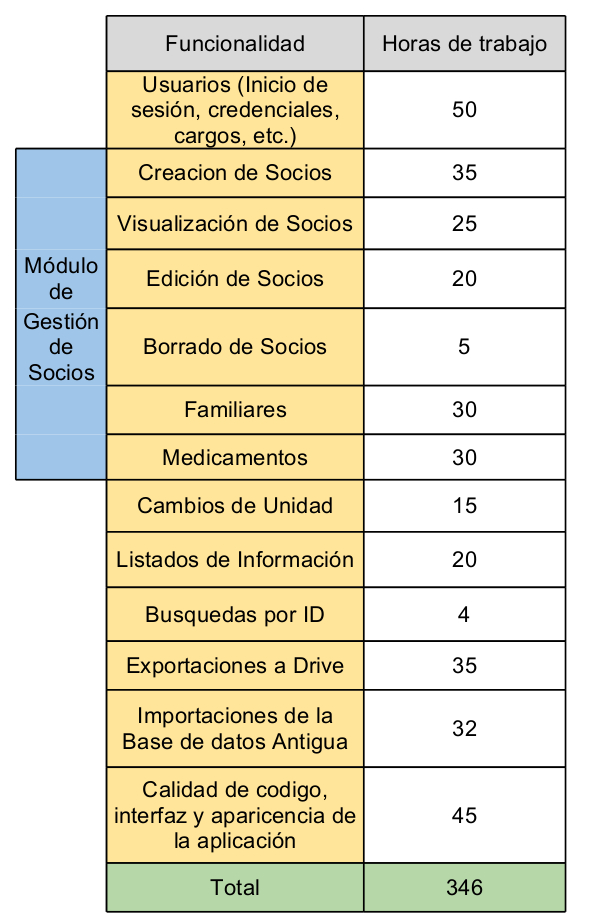
\includegraphics[width=0.65\textwidth]{images/presupuesto.jpg}
\caption{Números de horas totales y de desarrollo que se llevaron a cabo en el proyecto}
\label{fig:presupuesto}
\end{center}
\end{figure}

\newpage

Por otro lado, destacamos el porcentaje de investigación que tuvo cada funcionalidad, de esta manera podemos ver que funcionalidad fue más complicada de
desarrollar según su porcentaje de investigación. Y para finalizar se descontaron estas horas de investigación para obtener el número neto de horas de desarrollo de cada funcionalidad, cuya suma sera el 
total de horas exclusivas de desarrollo, que son las horas que se le facturaran al cliente (166,4 horas).\\


Dicho esto la tarifa por de desarrollo establecida en este proyecto es de \textbf{12 euros} la hora.\\

\bigskip

Por tanto la aplicación \textbf{GScout} tendrá un precio de: {\Huge \textbf{1996,90 euros}}\\




%%%%%%%%%%%%%%%%%%%%%%%%%%%%%%%%%%%%%%%%%%%%%%%%%%%%%%%%%%%%%%%%%%%%%%%%%%%%%%%

%%%%%%%%%%%%%%%%%%%%%%%%%%%%%%%%%%%%%%%%%%%%%%%%%%%%%%%%%%%%%%%%%%%%%%%%%%%%%%%
\newpage{\pagestyle{empty}\cleardoublepage}
\thispagestyle{empty}
\begin{appendix}

\chapter{Título del Apéndice 1}
\label{appendix:1}
\section{Algoritmo XXX}
\label{Apendice1:XXX}

\begin{center}
\begin{footnotesize}
\begin{verbatim}

***********************************************************************************
*
* Fichero .h
*
***********************************************************************************
*
* AUTORES
*   
*
* FECHA
*   
*
* DESCRIPCION
*   
*
************************************************************************************/

\end{verbatim}
\end{footnotesize}
\end{center}

\section{Algoritmo YYY}
\label{Apendice1:YYY}

\begin{center}
\begin{footnotesize}
\begin{verbatim}


/***********************************************************************************
 *
 * Fichero .h
 *
 ***********************************************************************************
 *
 * AUTORES
 *
 * FECHA
 *
 * DESCRIPCION
 *
 *
 ************************************************************************************/

\end{verbatim}
\end{footnotesize}
\end{center}


\chapter{Título del Apéndice 2}
\label{appendix:2}
\section{Otro apendice: Seccion 1}
\label{Apendice2:label}

\begin{center}
\begin{footnotesize}

\begin{verbatim}
Texto
\end{verbatim}

\end{footnotesize}
\end{center}

\section{Otro apendice: Seccion 2}
\label{Apendice2:label2}

\begin{center}
\begin{footnotesize}

\begin{verbatim}
Texto
\end{verbatim}


\end{footnotesize}
\end{center}


\end{appendix}

%%%%%%%%%%%%%%%%%%%%%%%%%%%%%%%%%%%%%%%%%%%%%%%%%%%%%%%%%%%%%%%%%%%%%%%%%%%%%%%
\addcontentsline{toc}{chapter}{Bibliografía}
\bibliographystyle{plain}

\bibliography{memtfg}
\nocite{*}

%%%%%%%%%%%%%%%%%%%%%%%%%%%%%%%%%%%%%%%%%%%%%%%%%%%%%%%%%%%%%%%%%%%%%%%%%%%%%%%

\end{document}
